\section{An algorithm to decide type bisimilarity}
\label{sec:algorithm}

% Recall the type bisimulation problem for context-free session types.

% \begin{quote}
%   Given context-free session types $S$ and $T$, the type equivalence
%   problem consists in deciding if types $S$ and $T$ are equivalent,
%   i.e., $S \TypeEquiv T$.
% \end{quote}

This section presents an algorithm to decide whether two types are in
a bisimulation relation. In the process we also provide an algorithm
to decide the equivalence of simple context-free languages.
%
The algorithm comprises three stages. It
starts by converting types into grammars and then streamlines the
grammar by pruning unreachable symbols in productions. The last stage
explores an expansion tree, alternating between simplification and
expansion operations, until either finding an empty node---case in
which it decides positively---or failing to expand a node---case in
which it decides negatively.

\subsection{Converting types to grammars}
\label{subsec:typeToGrammar}

A context-free grammar in Greibach normal form is a pair
$(X,\productions)$ where~$X$ is the \emph{start symbol}
and~$\mathcal P$ a \emph{set of productions} of the form
$Y \rightarrow a\vec Z$ (we do not allow productions of the form
$X \rightarrow\varepsilon$). Type variables are the \emph{non-terminal
  symbols} and LTS labels the \emph{terminal symbols}. We call
\emph{words} to sequences of type variables~$\vec X$, and denote
by~$\varepsilon$ the empty word.
%
The grammars we are interested in are \emph{simple}: for each
non-terminal symbol~$X$ and each terminal symbol~$a$, there is at most
one production of the form
$X \rightarrow a\vec Y$~\cite{simpleGrammar}. 

Grammars in Greibach Normal Form naturally induce an LTS by taking
sequences of non-terminal symbols~$\vec X$ as states, terminal
symbols~$a$ as the set of actions, and the transition relation
$\LTSderivesP$ defined as $X\vec Y\LTSderivesP \vec Z\vec Y$ when
$X \rightarrow a\vec Z \in\productions$.
% \vv{reference here}
The associated bisimulation is denoted by $\ProdEquiv$.

Given a context-free session type $S$, the algorithm starts by
inserting an initial production of the form
$X_S \rightarrow \,\initialProd\,(\toGrammarf\,S)$ in the set of
productions.
%
Function \lstinline|toGrammar| (Listing~\ref{lst:toGrammar}) returns a
sequence of non-terminal symbols, while computing the remaining
productions.
%
It uses a predicate \lstinline|isChecked| $S$ to determine whether $S$
is terminated, that is whether \DONE S.
%
The algorithm keeps the set of productions and an integer (to generate
fresh non-terminal symbols) in the monadic state
\lstinline{TransState}. It uses the following functions to manipulate
state.
%
\begin{itemize}
\item \lstinline{freshVar} returns a fresh non-terminal symbol (a type
  variable);
\item \lstinline{addProduction}$\,X\,a\,\vec Y$ updates the state by inserting
  the production $X\rightarrow a\vec Y$;
% \item \lstinline{insertVisited} marks a non-terminal symbol as visited;
% \item \lstinline{isVisited} identifies whether the given non-terminal symbol
%   was previously visited;
% \item \lstinline{subst} $X\,T\,S$ replaces the occurrences of~$X$
%   by~$T$ in~$S$;
\item \lstinline|getTransitions|$\,X$ retrives the transitions
  from~$X$ (a map from non-terminal symbols~$a$ to sequences~$\vec Y$
  of type variables).
\end{itemize}

% In Listing~\ref{lst:toGrammar}, type $\skipk$ is represented by
% \lstinline{Skip}, \lstinline{Message p b} stands for types of the form
% $\sharp B$,
% %\lstinline{VarLabel} stands for variables,
% \lstinline{Semi} represents sequential composition,
% \lstinline{Rec} represents recursive types, and
% \lstinline{Choice} stands for the choice operators $\oplus$ and
% $\&$. \vv{cut? looks obvious, and there is many more related things to say}

\begin{lstlisting}[
  caption={Haskell code for stage 1: the conversion of types into grammars},
  label={lst:toGrammar},
  captionpos=b]
type Transitions = Map.Map LTSLabel [TypeVar]
type Productions = Map.Map TypeVar Transitions
type Visited = Set.Set TypeVar
type TransState = State (Productions, Int)

toGrammar :: Type -> TransState [TypeVar]
toGrammar Skip =
  return []
toGrammar (Message p b) = do
  y <- freshVar
  addProduction y (MessageLabel p b) []
  return [y]
toGrammar (Choice c m) = do
  y <- freshVar
  mapM_ (assocsToGrm y c) (Map.assocs m)
  return [y]
toGrammar (Semi t u) = do
  xs <- toGrammar t
  ys <- toGrammar u
  return (xs ++ ys)
toGrammar (Rec x t) = do
  zs <- toGrammar t
  if null zs
    then return []
    else do
      m <- getTransitions (head zs)
      addProductions x (Map.map (++ tail zs) m)
      return [x]
toGrammar (Var x) =
  return [x]

assocsToGrm :: TypeVar -> ChoiceView -> (TypeLabel,Type) -> TransState ()
assocsToGrm y c (l, t) = do
  xs <- toGrammar t
  addProduction y (ChoiceLabel c l) xs
\end{lstlisting}

%%% Local Variables:
%%% mode: latex
%%% TeX-master: "main"
%%% End:


Notice that function \lstinline|toGrammar| terminates on all inputs and
that the resulting set of productions is finite, because recursion is
always on subterms.
%
Furthermore, due to the deterministic nature of the LTS,
\lstinline|toGrammar| returns a simple grammar.
%
% , context-free session types are always converted into \emph{simple
%   grammars}~\cite{baeten1993decidability}, i.e., context-free grammars
% in Greibach normal form such that, for each non-terminal symbol $X$
% and terminal symbol $a$, there is at most one production of the form
% $X\rightarrow a \enspace \vec Y$.
%
One can obtain a unique set of productions for two types by
ensuring that fresh variables do not overlap.

\begin{example}
\label{ex:productions}
Consider the following context-free session types:
%
\begin{equation*}
\begin{array}{lll}
    S & \triangleq & (\mu x . \&\{n: x;x;?\intk, \ell: ?\intk\});(\mu z . !\intk ; z;z)\\
    T & \triangleq & (\mu y . \&\{n: y;y, \ell: ?\skipk\};?\intk);(\mu w. !\intk ; w)
\end{array}
\end{equation*}
%
Function \lstinline{toGrammar}, when applied to $S$ and $T$, produces
the following productions.
\begin{center}
  \begin{tabular}{l l}
    \multicolumn{2}{c}{Productions for type $S$}\\ \hline
    $X_S \rightarrow \,\initialProd\, X_1 X_4$ &$X_2 \rightarrow \,? \intk$\\
    $X_1 \rightarrow \& n\, X_1 X_1 X_2$&$X_3 \rightarrow \,? \intk$\\
    $X_1 \rightarrow \& \ell\, X_3$ &$X_4 \rightarrow \,!\intk\, X_4 X_4$\\
  \end{tabular} \qquad
  \begin{tabular}{l l}
    \multicolumn{2}{c}{Productions for type $T$}\\ \hline
    $Y_T \rightarrow \,\initialProd\, Y_1 Y_3 $&$Y_2 \rightarrow \,? \intk$\\
    $Y_1 \rightarrow \& n\, Y_1 Y_1 Y_2 $&$Y_3 \rightarrow \,!\intk\, Y_3$\\
    $Y_1 \rightarrow \& \ell \,Y_2 $ &
  \end{tabular}
\end{center}
\end{example}

\subsection{Pruning unnormed productions}
\label{subsec:prune}

For $\vec a$ a sequence of non-terminal symbols $a_1,\ldots, a_k$
($k\ge1$), write $\vec Y \LTSderivesP[\vec a] \vec Z$ when
$\vec Y \LTSderivesP[a_1] \cdots \LTSderivesP[a_k] \vec Z$.
%
We say that $\vec Y$ is \emph{normed} when
$\vec Y \LTSderivesP[\vec a] \varepsilon$ for some~$\vec a$, and that
$\vec Y$ is \emph{unnormed} otherwise.
%
When $\vec Y$ is normed, the \emph{minimal path} of $\vec Y$ is the
shortest~$\vec a$ such that $\vec Y \LTSderivesP[\vec a]
\varepsilon$.
%
In this case, the \emph{norm} of $\vec Y$, denoted by $|\vec Y|$, is
the length of~$\vec a$.

% Using the same approach as~\cite{DBLP:journals/iandc/ChristensenHS95} on
% the definition of (un)normed processes, we say that a sequence of symbols
% $\vec Y$ is \emph{normed} if there are labels $a_1,\ldots, a_k$
% such that:
% \begin{equation}
% \label{eq:path}
% 	\vec Y \rightarrow a_1\enspace Y_1 \rightarrow \cdots \rightarrow a_k
% 	\rightarrow \varepsilon.
% \end{equation}
% $\vec Y$ is said to be \emph{unnormed} when it is not normed. If $\vec Y$
% is normed, we define its \emph{norm} as:
% \[ | \vec Y | = \underset{k}{\mathsf{min}} \{\vec Y \rightarrow a_1\enspace Y_1
% \rightarrow \cdots \rightarrow a_k \rightarrow \varepsilon \}.\]
% A \emph{minimal path} for a normed sequence of symbols $\vec Y$ is a sequence of
% labels $\vec a = a_1,\ldots,a_k$ as in~\eqref{eq:path} such that
% $k = | \vec Y |$. To ease notation, we will also represent~\eqref{eq:path} as
% $\vec Y \xrightarrow{\vec a} \varepsilon$.

As observed by Christensen et
al.~\cite{DBLP:journals/iandc/ChristensenHS95}, any unnormed sequence
of symbols $\vec Y$ is bisimilar to its concatenation with any other
symbols, that is, if $\vec Y$ is unnormed, then
$\vec Y \ProdEquiv \vec YX$.
%
% \begin{equation}
%\label{unnormed}
%\text{ if } \vec Y \text{ is unnormed, then } \vec Y \sim \vec Y X.
%\end{equation}
%
We use this fact
% Upon the definition of the productions underlying the context-free session types,
% our algorithm builds upon~\eqref{unnormed}
to prune out unreachable symbols in unnormed sequences of symbols. The
code is in Listing~\ref{lst:prune}.
%
%\vv{normedWord needs to be rewritten}

\begin{lstlisting}[
  caption={Haskell code for stage 2: pruning unnormed productions},
  label={lst:prune},
  captionpos=b
  ]
prune :: Productions -> Productions
prune p = Map.map (Map.map (pruneWord p)) p

pruneWord :: Productions -> [TypeVar] -> [TypeVar]
pruneWord p = foldr (\x ys -> if normed p x then x:ys else [x]) []

normed :: Productions -> TypeVar -> Bool
normed p x = normedWord p Set.empty [x]

normedWord :: Productions -> Visited -> [TypeVar] -> Bool
normedWord _ _ []     = True
normedWord p v (x:xs) =
  x `Set.notMember` v &&
  any (normedWord p v') (Map.elems (transitions p (x:xs)))
  where v' = if any (x `elem`) (Map.elems (transitions p [x]))
               then Set.insert x v else v
\end{lstlisting}

\begin{example}
  \label{ex:prune}
  Recall Example~\ref{ex:productions} and notice that both
  $X_S$ and
  $Y_T$ are unnormed. We can easily see that the last occurrence of
  $X_4$ in the last production for
  $S$ is unreachable. Hence, by pruning the productions for
  $S$ we get:
  %
  \begin{center}
    \begin{tabular}{l l l}
      \multicolumn{3}{c}{Pruned productions for type $S$}\\ \hline
      $X_S \rightarrow \,\initialProd\, X_1 X_4$ &
      $X_1 \rightarrow \& \ell\, X_3$  &
      $X_1 \rightarrow \& n\, X_1 X_1 X_2$
      \\
      $X_2 \rightarrow \,? \intk$ &
      $X_3 \rightarrow \,? \intk$ &
      $X_4 \rightarrow \,!\intk\, X_4$
    \end{tabular}
  \end{center}
\end{example}

\subsection{Building expansion trees}
\label{subsec:expand}

% We recall that, given two context-free session types $S$ and $T$, our main goal
% is to decide whether these types are equivalent or not. For this purpose,
% the algorithm we propose starts by applying algorithm presented in
% Listing~\ref{lst:toGrammar} to convert $S$ and $T$ into a grammar containing
% the productions derived from them. Afterwards, the algorithm in
% Listing~\ref{lst:prune} is used to streamline the grammars, by pruning
% unnormed sequences of symbols. Throughout this section we focus on the
% third and last step of the algorithm.

We base the third stage of the algorithm on the notion of
\emph{expansion tree} proposed by Jan{\v{c}}ar and
Moller~\cite{janvcar1999techniques}, an adaption of an idea by
Hirshfeld~\cite{hirshfeld1996bisimulation}. We say a set $N'$ of pairs
of words is an \emph{expansion} of $N$ if $N'$ is a minimal set such
that: for every pair $(\vec X, \vec Y) \in N$,
\begin{itemize}
\item if $\vec X \rightarrow a\vec X'$ then
  $\vec Y \rightarrow a\vec Y'$ with $(\vec X',\vec Y')\in N'$;
\item if $\vec Y \rightarrow a\vec Y'$ then
  $\vec X \rightarrow a \vec X'$ with $(\vec X',\vec Y')\in N'$.
\end{itemize}

An \emph{expansion tree} is built from nodes. Children nodes are
obtained by expansion from its parent node. Jan{\v{c}}ar and Moller
observed that expansion alone often leads to infinite trees. We then
alternate between expansion and simplification operations, until
either finding an empty node---case in which we decide equivalence
positively---or failing to expand a node---case in which we decide
equivalence negatively.
%
% The na\"ive proposal for an expansion tree considers that any
% children node is obtained by expansion from its parent
% node. Nevertheless, as Jan{\v{c}}ar and Moller observed, this would
% often lead to infinite expansion trees. Hence, we follow the
% proposal in~\cite{janvcar1999techniques} and let the expansion tree
% alternate between simplification and expansion operations until
% either finding an empty node---case in which we decide equivalence
% positively---or failing to expand a node---case in which we decide
% equivalence negatively.
%
We say that a branch is \emph{successful} if it is infinite or
finishes in an empty node, otherwise it is said to be
\emph{unsuccessful}.

%\paragraph*{Expansion step}
In the \emph{expansion step}, each node $N$ derives a single children
node, obtained as an expansion of $N$. As we are dealing with simple
grammars, no branching is expected in the expansion tree at this
step.
%
% \paragraph*{Simplification step}
The \emph{simplification step} consists on the application of the
following rules:
%
\begin{description}
\item[Reflexive rule:] Omit from a node any reflexive pair;
\item[Congruence rule:] Omit from a node $N$ any pair that belongs to
  the least congruence containing the ancestors of $N$;
  % \item {\bf Basic Process Algebra rules:} create sibling nodes for $N$
  % according to the following rules:
  % \begin{description}
\item[BPA1 rule:] If $(X_0 \vec X, Y_0 \vec Y)$ is in
  $N$ and $(X_0 \vec {X'}, Y_0 \vec {Y'})$ belongs to the ancestors of
  $N$, then create a sibling node for $N$ replacing
  $(X_0 \vec X, Y_0 \vec Y)$ by $(\vec X, \vec {X'})$ and
  $(\vec Y, \vec {Y'})$;
\item[BPA2 rule:] If $(X_0 \vec X, Y_0 \vec Y)$ is in $N$
  and $X_0$ and $Y_0$ are normed, then:
  \begin{description}
  \item[Case] $|X_0| \leq |Y_0|$: considering $\vec a$ as a minimal path
    for $X_0$ and $\vec Z$ a word such that
    $\vec Y_0 \LTSderivesP[\vec a] \vec Z$. Add a sibling node for
    $N$ including the pairs $(X_0 \vec Z, Y_0)$ and
    $(\vec X, \vec Z \vec Y)$ in place of $(X_0 \vec X, Y_0 \vec Y)$;
  \item[Case] $|X_0| > |Y_0|$: considering $\vec a$ as a minimal path for
    $Y_0$ and $\vec Z$ a word such that $\vec X_0 \LTSderivesP[\vec a] \vec
    Z$. Add a sibling node for $N$ including the pairs
    $(X_0 , Y_0 \vec Z )$ and $(\vec Z\vec X, \vec Y)$ in place of
    $(X_0 \vec X, Y_0 \vec Y)$.
  \end{description}
%		  \end{description}
%	\item {\bf Filtering rule:} remove any node containing a pair
%	       $(\vec X, \vec Y)$ such that $|\vec X|\neq |\vec Y|$.
\end{description}

Contrarily to expansion and to the reflexive and congruence
simplifications, \BPA\ rules promote branching in the expansion
tree. The number of children nodes generated by these rules is
finite~\cite{DBLP:journals/iandc/ChristensenHS95}.
%
Notice that the sibling nodes do not exclude the (often) infinite
branch resulting from successive expansions.

\subsection{Checking the bisimilarity of context-free session types}

% The algorithm to decide the equivalence of context-free session
% types capitalizes on the previous algorithms.

Given two context-free session types, function \lstinline|bisimilar|
in listing~\ref{lst:algorithm} starts by converting the two session
types into a grammar, which is then pruned. Function
\lstinline|convertToGrammar| (not shown) builds the initial monadic
state, and runs the algorithm of section~\ref{subsec:typeToGrammar} to
convert the session types given as parameters.
%
An expansion tree is computed afterwards, through an alternation of
expansion of children nodes and their simplification, using the
reflexive, congruence, and \BPA\ rules. This recursive procedure
terminates as soon as all nodes fail to expand and, thus, the queue is
empty, case in which the algorithm returns \lstinline|False|, or an
empty node is reached, case is which the algorithm returns
\lstinline|True|.
%
To avoid getting stuck in an infinite branch of the expansion tree, we
use a breadth-first search on the expansion tree. Upcoming nodes are
stored in a queue.

\begin{lstlisting}[
  caption={Haskell code for checking the bisimilarity of context-free
    session types},
  label={lst:algorithm},
  captionpos=b
  ]
type Node = Set.Set ([TypeVar], [TypeVar])
type Ancestors = Node
type NodeQueue = Queue.Queue (Node, Ancestors)
type NodeTransformation = Productions -> Ancestors -> Node -> Set.Set

bisimilar :: Type -> Type -> Bool
bisimilar t u = expand (prune p) [x] [y]
  where Grammar [x, y] p = convertToGrammar [t, u]

expand :: Productions -> NodeQueue -> Bool
expand ps q
  | Queue.null q = False 
  | Set.null n   = True
  | otherwise    = case expandNode ps n of
      Nothing -> expand ps (Queue.dequeue q)
      Just n' -> expand ps (simplify ps n' (Set.union a n) q)
  where (n,a) = Queue.front q

simplify :: Productions -> Node -> Ancestors -> NodeQueue -> NodeQueue
simplify ps n a q = foldr Queue.append (Queue.dequeue q) ns'
  where ns  = Set.singleton (n,a)
        ns' = if allNormed ps
               then foldr (apply ps) ns [reflex,congruence,bpa2]
               else foldr (apply ps) ns [reflex,congruence,bpa1,bpa2]
\end{lstlisting}

\begin{figure}[t!]
\centering
	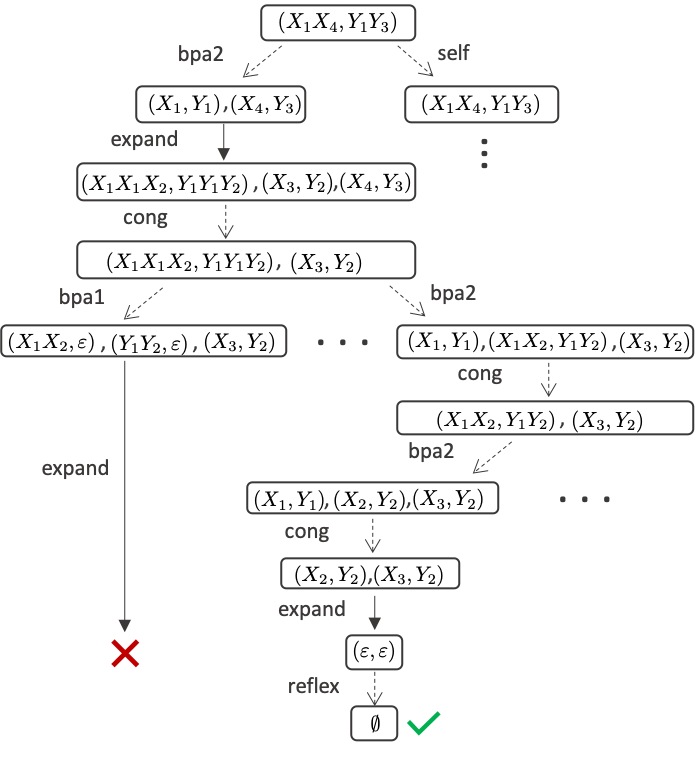
\includegraphics[width=8.5cm]{expansionTree}
	\caption{Expansion tree for the context-free session types $S$ and $T$
	introduced in Example~\ref{ex:productions}.}
	\label{fig:expansionTree}
\end{figure}

\begin{example}
  The expansion tree for our running example is
  in Figure~\ref{fig:expansionTree}. Once a successful
  branch is reached (the $\checkmark$ in the figure), the algorithm in
  Listing~\ref{lst:algorithm} decides that $S\TypeEquiv T$.
\end{example}

%%% Local Variables:
%%% mode: latex
%%% TeX-master: "main"
%%% End:
